\section{Empirical Evaluation}

We next test whether the CLOC-derived regularizers produce useful continual-learning behavior in practical settings. Unless stated otherwise, all EWC matrices are diagonal. We write U-IEWC for the empirical, uniformly weighted IEF aggregation with $h_n\equiv 1$, and GSS-IEWC for a weighted variant that applies the gradient-diversity principle of GSS to the normalized IEWC directions \citep{GSS}. The classification setting is ImageNet-R class-incremental learning with a pretrained ViT-B/16 and LoRA adapters, while the NLP setting is TRACE multiple-choice continual fine-tuning with Qwen2.5-3B and LoRA adapters. Thus, these two setups place the comparison in the recent line of parameter-efficient continual fine-tuning, including LoRA and recent continual LoRA methods \citep{LoRA,FRLoRA,CLLoRA,CLoRA}. We also evaluate non-LoRA fine-tuning of a pretrained CNN for VOC 15-5 semantic segmentation, and from-scratch training for long-horizon time-series forecasting and MNIST DDPM denoising. For each method and task type, we tune $\lambda$ to optimize the average performance metric across distributions; Appendix C gives the full training and tuning protocol, including the selected $\lambda$ and $\tau$ values.

\begin{table}[H]
\centering
\resizebox{\linewidth}{!}{%
\begin{tabular}{llccccc}
\toprule
Task type & Metric & Sequential & EF-EWC & EWC-DR & U-IEWC & GSS-IEWC \\
\midrule
Classification & Final avg. accuracy $\uparrow$ & 0.2896 $\pm$ 0.0405 & 0.5981 $\pm$ 0.0337 & 0.5687 $\pm$ 0.0263 & \textbf{0.6332 $\pm$ 0.0232} & 0.6250 $\pm$ 0.0263 \\
Classification & Avg. forgetting $\downarrow$ & 0.7066 $\pm$ 0.0466 & 0.3595 $\pm$ 0.0378 & 0.3933 $\pm$ 0.0286 & \textbf{0.3142 $\pm$ 0.0250} & 0.3285 $\pm$ 0.0278 \\
NLP & Final avg. score $\uparrow$ & 0.5760 $\pm$ 0.0027 & 0.5972 $\pm$ 0.0020 & 0.5972 $\pm$ 0.0059 & 0.5938 $\pm$ 0.0034 & \textbf{0.6272 $\pm$ 0.0080} \\
NLP & Avg. forgetting $\downarrow$ & 0.1139 $\pm$ 0.0111 & 0.0762 $\pm$ 0.0034 & 0.0781 $\pm$ 0.0109 & 0.0820 $\pm$ 0.0122 & \textbf{0.0046 $\pm$ 0.0079} \\
Forecasting & Final avg. MSE $\downarrow$ & 0.2733 $\pm$ 0.0065 & 0.2388 $\pm$ 0.0021 & -- & 0.2418 $\pm$ 0.0038 & \textbf{0.2383 $\pm$ 0.0007} \\
Forecasting & Avg. MSE forgetting $\downarrow$ & 0.0535 $\pm$ 0.0081 & \textbf{0.0140 $\pm$ 0.0020} & -- & 0.0191 $\pm$ 0.0047 & 0.0147 $\pm$ 0.0021 \\
Segmentation & Final all mIoU $\uparrow$ & 0.0917 $\pm$ 0.0061 & 0.0946 $\pm$ 0.0040 & 0.3080 $\pm$ 0.0307 & \textbf{0.4678 $\pm$ 0.0568} & 0.4274 $\pm$ 0.0574 \\
Segmentation & Base-class forgetting $\downarrow$ & 0.7135 $\pm$ 0.0114 & 0.7131 $\pm$ 0.0166 & 0.4471 $\pm$ 0.0447 & \textbf{0.2418 $\pm$ 0.0965} & 0.2925 $\pm$ 0.0839 \\
Diffusion & Final avg. denoising MSE $\downarrow$ & 0.0676 $\pm$ 0.0029 & 0.0296 $\pm$ 0.0013 & -- & 0.0298 $\pm$ 0.0014 & \textbf{0.0293 $\pm$ 0.0013} \\
Diffusion & Denoising-MSE forgetting $\downarrow$ & 0.0503 $\pm$ 0.0002 & \textbf{-0.0006 $\pm$ 0.0020} & -- & 0.0001 $\pm$ 0.0024 & -0.0003 $\pm$ 0.0020 \\
\bottomrule
\end{tabular}
}
\caption[Main continual-learning results]{Main continual-learning results. The objective used for tuning is the final average performance across distributions; forgetting is reported separately as a retention measure. Higher is better for accuracy, score, and mIoU; lower is better for MSE and forgetting.}
\label{tab:main-empirical-results}
\end{table}

Overall, Table \ref{tab:main-empirical-results} separates the joint performance objective from the forgetting metric. U-IEWC gives the strongest ImageNet-R retention and average accuracy. In turn, GSS-IEWC gives the strongest TRACE result and the lowest average forecasting MSE, while EF-EWC is slightly better on forecasting forgetting. On VOC 15-5, U-IEWC gives the clearest gain over EF-EWC and EWC-DR. In DDPM denoising, the tuned regularizers are close; GSS-IEWC has the lowest average denoising MSE, and EF-EWC has the smallest measured forgetting within the reported variance.

\begin{figure}[H]
\centering
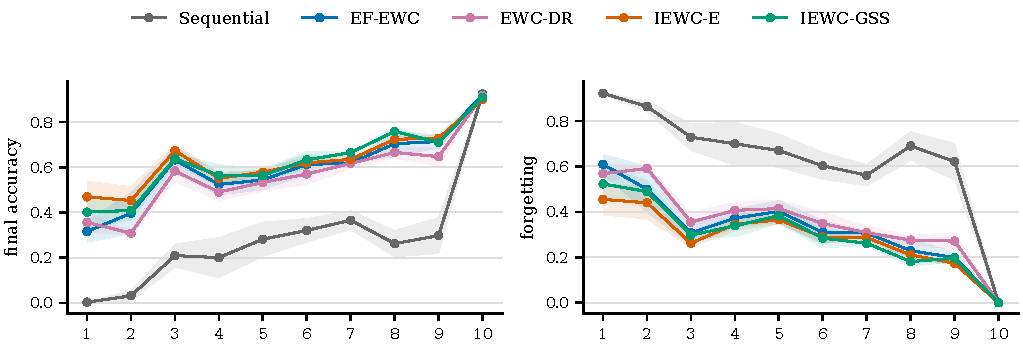
\includegraphics[width=0.65\linewidth]{figures/classification_distribution_retention.pdf}
\caption[ImageNet-R distribution retention]{ImageNet-R distribution retention. The left panel shows the final accuracy on each distribution after the full sequence; the right panel shows the corresponding forgetting. U-IEWC and GSS-IEWC improve retention across most distributions relative to EF-EWC, while sequential training forgets the early distributions almost entirely.}
\label{fig:classification-distribution-retention}
\end{figure}

At the distribution level, Figure \ref{fig:classification-distribution-retention} breaks the classification result down by distribution. The retained accuracy is not concentrated in a single late distribution: the IEWC variants reduce forgetting across the early and middle parts of the sequence, which is the regime where sequential fine-tuning fails most visibly.

\begin{figure}[H]
\centering
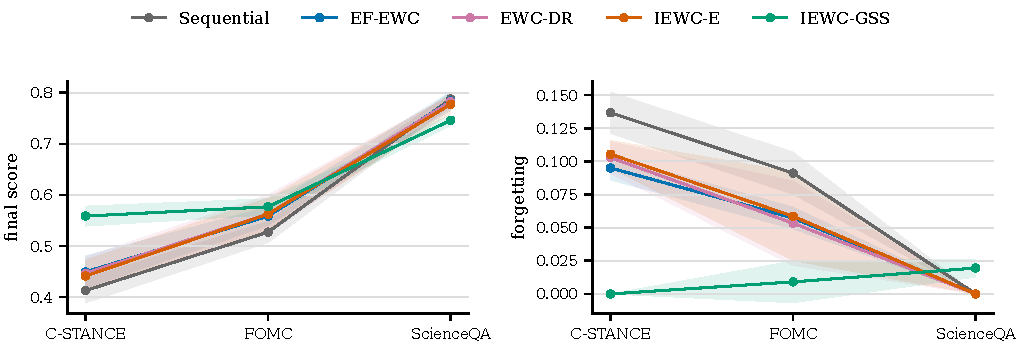
\includegraphics[width=0.65\linewidth]{figures/nlp_distribution_retention.pdf}
\caption[TRACE distribution retention]{TRACE distribution retention. The plot reports the final multiple-choice score and forgetting for C-STANCE, FOMC, and ScienceQA after sequential LoRA fine-tuning of Qwen2.5-3B. GSS-IEWC preserves the earlier NLP distributions while keeping competitive performance on the final distribution.}
\label{fig:nlp-distribution-retention}
\end{figure}

Similarly, the TRACE retention profile in Figure \ref{fig:nlp-distribution-retention} explains the table-level gain of GSS-IEWC. The weighted aggregation mainly changes the stability side of the tradeoff: it reduces forgetting on C-STANCE and FOMC while leaving ScienceQA in the same range as the other regularized methods.

\begin{figure}[H]
\centering
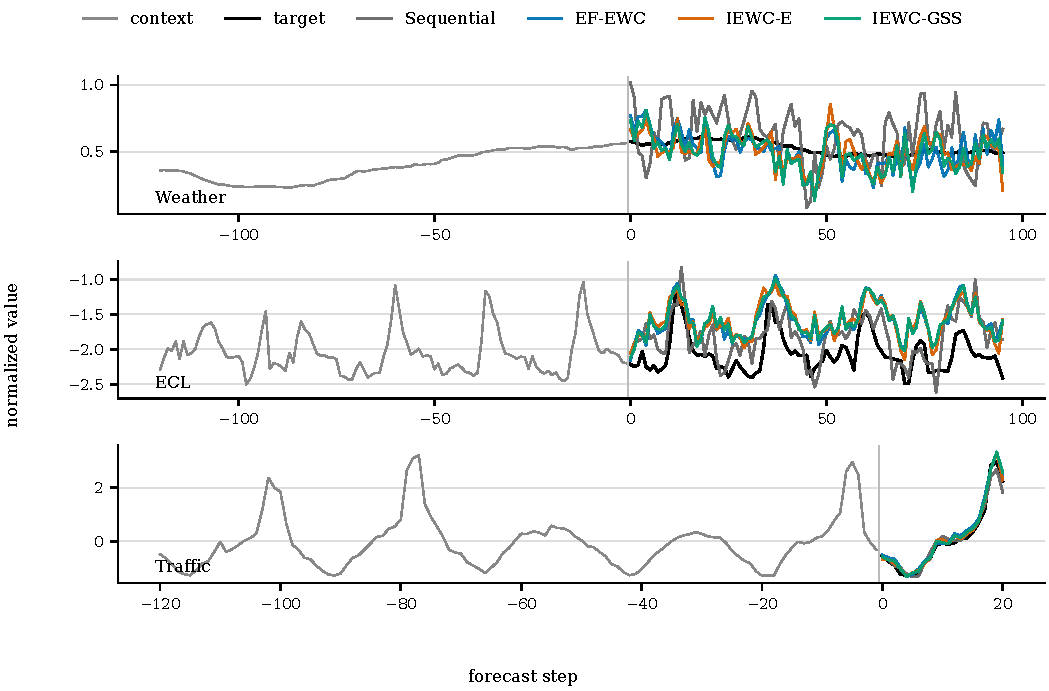
\includegraphics[width=0.75\linewidth]{figures/forecast_rollouts_longhorizon_tasknorm_selected.pdf}
\caption[Forecasting rollout comparison]{Forecasting rollout comparison. Each panel shows one held-out rollout from the corresponding forecasting distribution. The gray curve is the observed context, the black curve is the target horizon, and colored curves are method predictions after the full continual sequence.}
\label{fig:forecast-rollouts}
\end{figure}

For visual inspection and qualitative analysis, Figure \ref{fig:forecast-rollouts} adds individual forecasts. We can see that forgetting significantly affects all methods, while GSS-IEWC retains the most target trajectory structure at the first task and stays close to EF-EWC on later tasks.

In addition, the output-geometry parameter $\Gamma$ is evaluated separately in the DDPM setting. Replacing the Euclidean output metric with a sliced-Wasserstein surrogate lowers old-output sliced-Wasserstein drift relative to Euclidean U-IEWC ($9.4409\pm7.2517$ versus $14.1026\pm12.2220$), while keeping final average denoising MSE close to U-IEWC ($0.0301\pm0.0012$ versus $0.0298\pm0.0014$).

Finally, we tested FROMP-derived sample weighting \citep{FROMP} as a second alternative to the empirical weighting, with mixed results: on ImageNet-R, IEWC-FROMP reaches $0.6365\pm0.0165$ final average accuracy and $0.3068\pm0.0170$ forgetting, slightly ahead of GSS-IEWC; on VOC 15-5, it reaches only $0.3351\pm0.0742$ final all-mIoU and $0.4064\pm0.1122$ base-class forgetting, below U-IEWC and GSS-IEWC.

For reproducibility, Appendix C gives the experimental protocol, the programmatic $\lambda$ search, a damping sensitivity curve, and the effective summand-norm distributions. Appendix D connects the contamination model of Appendix B to a controlled label-noise experiment and reports the resulting accuracy and importance-matrix stability.

\subsection*{Code Release}

We release an accompanying repository with a readily usable IEWC implementation. The \texttt{IEWCConfig} class encapsulates the four-tuple parametrization introduced above. The same configuration interface is used by the diagonal and low-rank IEWC paths and by the empirical scripts, including the FACIL-based CIFAR-100 checks and the larger ImageNet-R, TRACE, forecasting, segmentation, and diffusion runs. The repository is available at \url{https://github.com/Axym-Labs/iewc}.
